\documentclass{article}

\setlength\parindent{0pt}

\usepackage{../preamble/factory, ../preamble/font, ../preamble/math, ../preamble/math_font, ../preamble/style, ../preamble/theorem}

\newtheorem{thr}{Uppgift}

\begin{document}

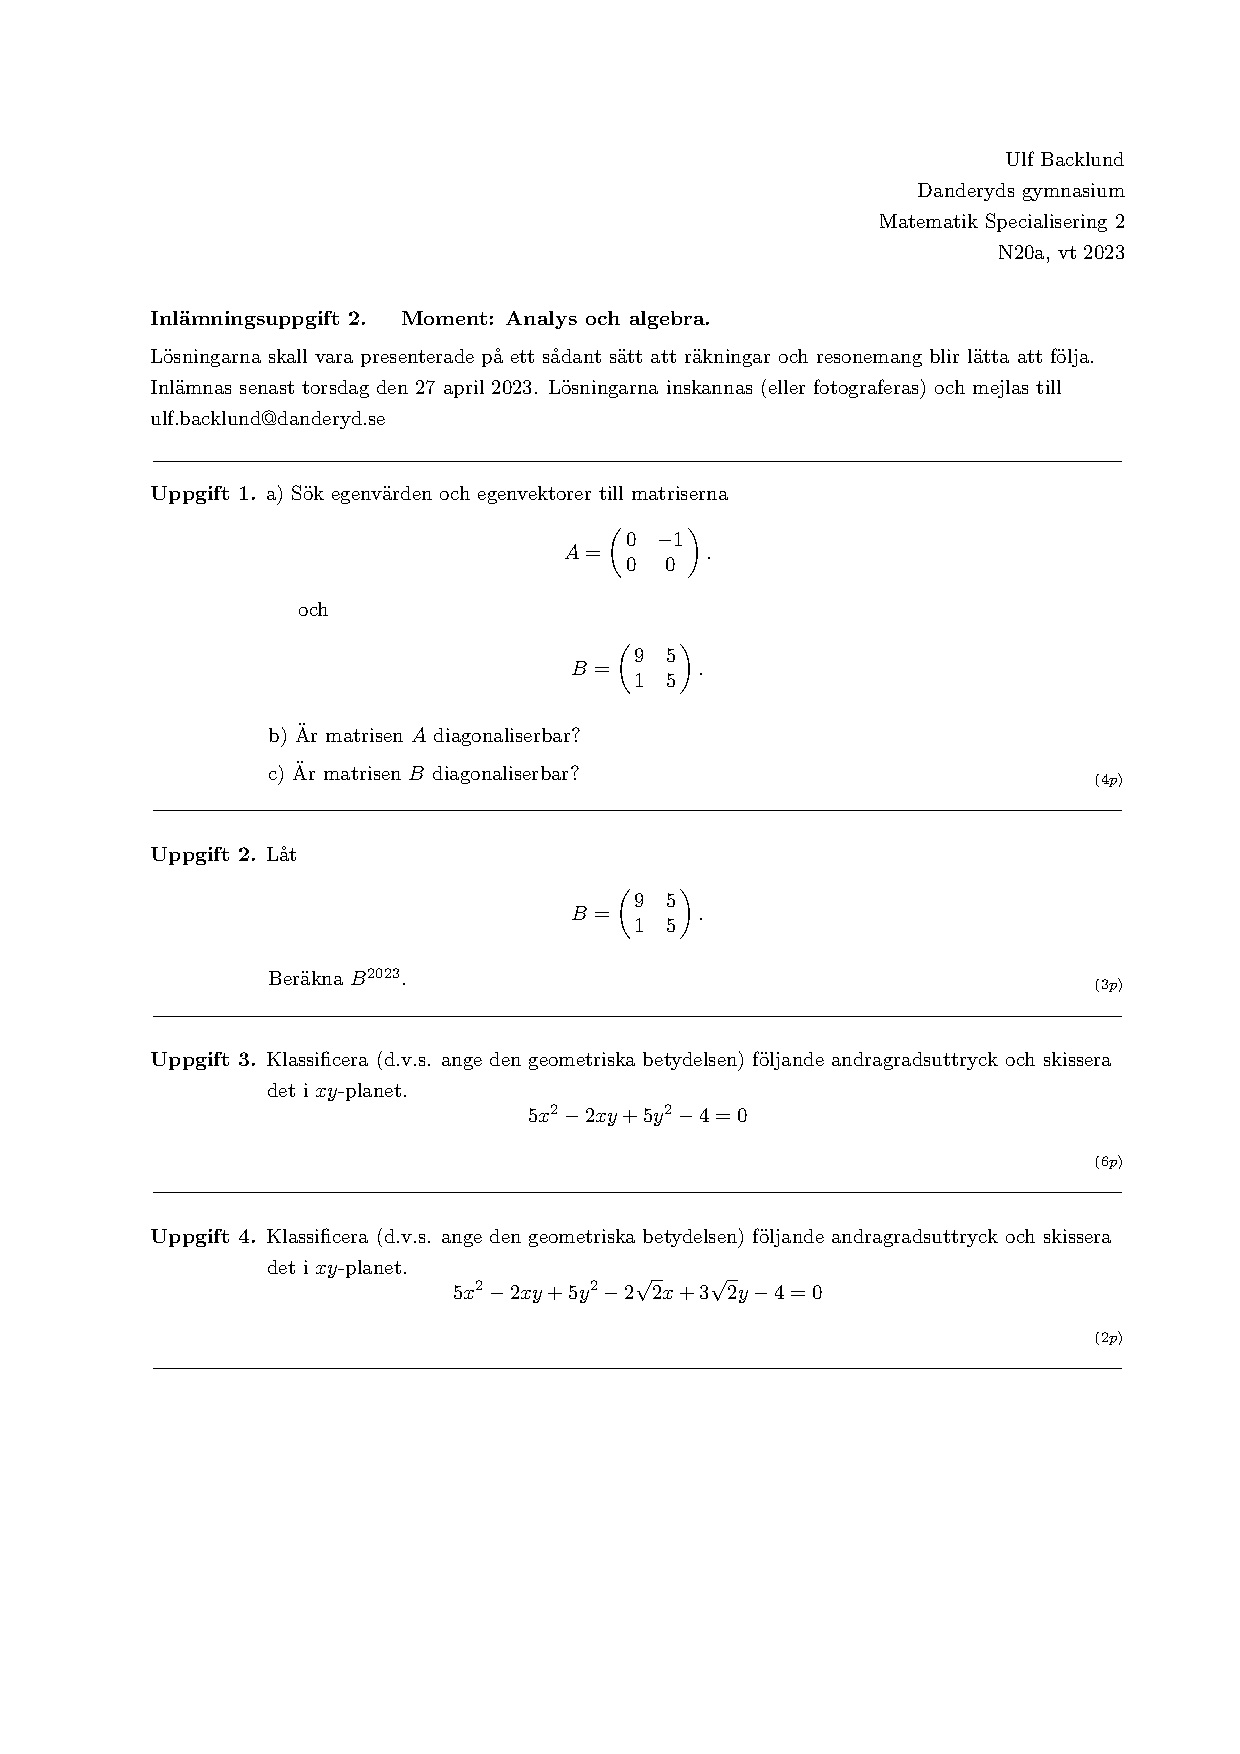
\includepdf{homework_2}

\newpage

\centerline{\large Matematik specialisering 2 inlämning 2}

\vskip 0.1cm

\centerline{\scriptsize Adam Amanbaev}

\vskip 1cm

\begin{thr}
\end{thr}

\begin{enumerate}
    \item[a)] Karakteristiska ekvationen ger följande:

        $$
        det(A-\lambda E)=0 
        \Ekv 
        \det\begin{pmatrix}
            0-\lambda & -1-0 \\
            0-0 & 0-\lambda 
        \end{pmatrix}
        =0
        \Imp
        (-\lambda)^2=0
        \Imp
        \lambda=0
        $$

        \vskip 0.3cm

        Det enda egenvärdet för matrisen $A$ är alltså $\lambda=0$.

        $$
        \therefore \; (A-\lambda E)X=0 
        \Ekv
        \begin{pmatrix}
            0 & -1 \\
            0 & 0
        \end{pmatrix}
        \begin{pmatrix}
            x_{1} \\
            x_{2}
        \end{pmatrix}
        =
        \begin{pmatrix}
            0 \\
            0
        \end{pmatrix}
        \Imp
        \begin{cases}
            -x_{2}=0 \\
            0=0
        \end{cases}
        $$
        
        \vskip 0.3cm

        $$
        \Imp
        \begin{cases}
            x_{2}=0 \\
            x_{1}=t, \; t \in \R
        \end{cases}
        $$

        \vskip 0.2cm

        Vi får egenvektorerna $\; X=\begin{pmatrix} 
           t \\
           0
        \end{pmatrix}, \; t\in\R
        $ för matrisen $A$.

        \vskip 0.3cm

        På samma vis får vi egenvärdena och egenvektorerna för matris $B$:

        \vskip 0.3cm

        $$
        det(B-\lambda E)=0 
        \Ekv 
        \det\begin{pmatrix}
            9-\lambda & 5-0 \\
            1-0 & 5-\lambda 
        \end{pmatrix}
        =0
        \Imp
        (9-\lambda)(5-\lambda)-5=0
        $$

        \vskip 0.3cm

        $$
        \Imp
        \lambda^2-14\lambda+40=0
        \Imp
        \lambda=7\pm3
        $$

        \vskip 0.3cm

        $$
        \therefore \; (A-\lambda E)X=0 
        \Ekv
        \begin{pmatrix}
            9-(7\pm3) & 5 \\
            1 & 5-(7\pm3)
        \end{pmatrix}
        \begin{pmatrix}
            x_{1} \\
            x_{2}
        \end{pmatrix}
        =
        \begin{pmatrix}
            0 \\
            0
        \end{pmatrix}
        $$

        \newpage

        $$
        \Imp
        \begin{cases}
            9x_{1}-(7\pm3)x_{1}+5x_{2}=0 \\
            x_{1}+5x_{2}-(7\pm3)x_{2}=0
        \end{cases}
        $$

        \vskip 0.3cm

        Fall 1 (-):

        \vskip -0.2cm

        $$ 
        \begin{cases}
            5x_{1}+5x_{2}=0 \\
            x_{1}+x_{2}=0
        \end{cases}
        \Ekv
        \begin{cases}
            x_{1}=-x_{2} \\
            0=0
        \end{cases}
        \Imp
        \begin{cases}
            x_{1}=-t \\
            x_{2}=t
        \end{cases}
        t\in\R
        \Imp
        X_{1}=
        \begin{pmatrix}
            -t \\
            t
        \end{pmatrix}
        $$

        \vskip 0.2cm

        Fall 2 (+):

        \vskip -0.2cm

        $$
        \begin{cases}
            -x_{1}+5x_{2}=0 \\
            x_{1}-5x_{2}=0
        \end{cases}
        \Ekv
        \begin{cases}
            x_{1}=5x_{2} \\
            0=0
        \end{cases}
        \Imp
        \begin{cases}
            x_{1}=5t \\
            x_{2}=t
        \end{cases}
        t\in\R
        \Imp
        X_{2}=
        \begin{pmatrix}
            5t \\
            t
        \end{pmatrix}
        $$

        \vskip 0.5cm

        $\therefore \;$ Matris $A$ har egenvärdet $\lambda=0$ och egenvektorerna $X=\begin{pmatrix} t \\ 0 \end{pmatrix}=t \; \begin{pmatrix} 1 \\ 0 \end{pmatrix}, \; t\in\R$

        \vskip 0.1cm

        medan matris $B$ har egenvärdena $\lambda_{1}=4 \Och \lambda_{2}=10$ och egenvektorerna

        \vskip 0.2cm

        $X_{1}=\begin{pmatrix} -t \\ t \end{pmatrix}=t \; \begin{pmatrix} -1 \\ 1 \end{pmatrix} \Och X_{2}=\begin{pmatrix} 5t \\ t \end{pmatrix}=t \; \begin{pmatrix} 5 \\ 1 \end{pmatrix}, \; t \in \R$

        \vskip 1cm

    \item[b)] För att 2x2 matrisen $A$ ska vara diagonaliserbar behöver den ha åtminstone två linjärt oberoende egenvektorer. Vi såg dock att den endast har en linjärt oberoende egenvektor vilket gör att $A$ inte är diagonaliserbar.

        \vskip 0.5cm

    \item[c)] Precis som matris $A$ behöver matris $B$ ha åtminstone två linjärt oberoende egenvektorer för att vara diagonaliserbar. $B$ har till exempel egenvektorerna $\begin{pmatrix} -1 \\ 1 \end{pmatrix}$ och $\begin{pmatrix} 5 \\ 1 \end{pmatrix}$ som är linjärt oberoende och därför är $B$ diagonaliserbar.
\end{enumerate}

\newpage

\begin{thr}
Beräkna $B^{2023}$
\end{thr}

Från uppgift 1 vet vi att matrisen $B=\begin{pmatrix} 9 & 5 \\ 1 & 5 \end{pmatrix}$ har egenvärdena $\lambda_{1}=4 \Och \lambda_{2}=10$ och

\vskip 0.1cm

egenvektorerna $X_{1}=\begin{pmatrix} -t \\ t \end{pmatrix}=t \; \begin{pmatrix} -1 \\ 1 \end{pmatrix} \Och X_{2}=\begin{pmatrix} 5t \\ t \end{pmatrix}=t \; \begin{pmatrix} 5 \\ 1 \end{pmatrix} \; t \in \R$. Vi vet därmed att 

\vskip 0.1cm

matrisen $A$ är diagonaliserbar ty den har två linjärt oberoende egenvektorer $\begin{pmatrix} -1 \\ 1 \end{pmatrix}$ och $\begin{pmatrix} 5 \\ 1 \end{pmatrix}$. Insättning av dessa egenvektorer och egenvärdena ovan ger följande:

\vskip 0.3cm

$$
\therefore 
\; 
D=
\begin{pmatrix}
    4 & 0 \\
    0 & 10 
\end{pmatrix}
\Och
T=
\begin{pmatrix}
    -1 & 5 \\
    1 & 1 
\end{pmatrix}
\Och
T^{-1}=
\frac{1}{6}
\begin{pmatrix}
    -1 & 5 \\
    1 & 1 
\end{pmatrix}
$$

\vskip 0.3cm

$$
\therefore
\;
D=T^{-1}BT
$$

\vskip -0.2cm

$$
\Ekv
TD=TT^{-1}BT
\Ekv
TDT^{-1}=BTT^{-1}
\Ekv
B=TDT^{-1}
$$

$$
\therefore
\;
B^{2023}=(TDT^{-1})^{2023}=(TDT^{-1})(TDT^{-1})(TDT^{-1})...(TDT^{-1})
$$

$$
=_{Associativitet}
TD(T^{-1}T)D(T^{-1}T)D(T^{-1}T)...(T^{-1}T)DT^{-1}
$$

$$
=
TD^{2023}T^{-1}
$$

$$
\therefore
\;
B^{2023}=
\begin{pmatrix}
    -1 & 5 \\
    1 & 1
\end{pmatrix}
\begin{pmatrix}
    4^{2023} & 0 \\
    0 & 10^{2023} 
\end{pmatrix}
\frac{1}{6}
\begin{pmatrix}
    -1 & 5 \\
    1 & 1
\end{pmatrix}
$$

$$
=
\begin{pmatrix}
    -4^{2023} & 5 \times 10^{2023} \\
    4^{2023} & 10^{2023}
\end{pmatrix}
\frac{1}{6}
\begin{pmatrix}
    -1 & 5 \\
    1 & 1
\end{pmatrix}
$$

$$
=
\frac{1}{6}
\begin{pmatrix}
    4^{2023}+5 \times 10^{2023} & -5 \times 4^{2023}+5 \times 10^{2023} \\
    -4^{2023}+10^{2023} & 5 \times 4^{2023}+10^{2023}
\end{pmatrix}
$$

\newpage

\begin{thr}
Klassificera (d.v.s. ange den geometriska betydelsen) andragradsuttrycket $5x^2-2xy+5y^2-4=0$ och skissera det i xy-planet.
\end{thr}

Vi vill få bort $-2xy$ termen för att enklare kunna klassificera uttrycket vilket vi gör genom att diagonalisera matrisen $A=\begin{pmatrix} 5 & -1 \\ -1 & 5 \end{pmatrix}$ som även kan ses som en rotation i koordinatsystemet. Vi börjar med att hitta $A$:s egenvärden och egenvektorer med hjälp av karakteristiska ekvationen:

$$
det(A-\lambda E)=0 
\Ekv 
\det\begin{pmatrix}
    5-\lambda & -1-0 \\
    -1-0 & 5-\lambda 
\end{pmatrix}
=0
\Imp
(5-\lambda)^2=1
\Imp
\lambda=5\pm1
$$

$$
\therefore
\;
(A-\lambda E)X=0 
\Ekv
\begin{pmatrix}
    5-(5\pm1) & -1 \\
    -1 & 5-(5\pm1)
\end{pmatrix}
\begin{pmatrix}
    x_{1} \\
    x_{2}
\end{pmatrix}
=
\begin{pmatrix}
    0 \\
    0
\end{pmatrix}
$$

$$
\Imp
\begin{cases}
    5x_{1}-(5\pm1)x_{1}-x_{2}=0 \\
    -x_{1}+5x_{2}-(5\pm1)x_{2}=0
\end{cases}
$$

\vskip 0.2cm

Fall 1 (-):

\vskip -0.2cm

$$ 
\begin{cases}
    x_{1}-x_{2}=0 \\
    -x_{1}+x_{2}=0
\end{cases}
\Ekv
\begin{cases}
    x_{1}=x_{2} \\
    0=0
\end{cases}
\Imp
\begin{cases}
    x_{1}=t \\
    x_{2}=t
\end{cases}
t\in\R
\Imp
X_{1}=
\begin{pmatrix}
    t \\
    t
\end{pmatrix}
$$

\vskip 0.2cm

Fall 2 (+):

\vskip -0.2cm

$$ 
\begin{cases}
    -x_{1}-x_{2}=0 \\
    -x_{1}-x_{2}=0
\end{cases}
\Ekv
\begin{cases}
    x_{1}=-x_{2} \\
    0=0
\end{cases}
\Imp
\begin{cases}
    x_{1}=-t \\
    x_{2}=t
\end{cases}
t\in\R
\Imp
X_{2}=
\begin{pmatrix}
    -t \\
    t
\end{pmatrix}
$$

\vskip 0.3cm

$\therefore$ Matrisen $A$ har egenvärdena $\lambda_{1}=4 \Och \lambda_{2}=6$ och egenvektorerna $X_{1}=\begin{pmatrix} t \\ t \end{pmatrix}=t \; \begin{pmatrix} 1 \\ 1 \end{pmatrix} \Och X_{2}=\begin{pmatrix} -t \\ t \end{pmatrix}=t \; \begin{pmatrix} -1 \\ 1 \end{pmatrix}, \; t \in \R$.

\newpage

Vi skriver om första delen av andragradsuttryket på följande vis:

$$
5x^2-2xy+5y^2=K^{t}AK,
\text{  där}
\;
K=
\begin{pmatrix}
    x \\
    y
\end{pmatrix}
\Och
A=
\begin{pmatrix}
    5 & -1 \\
    -1 & 5
\end{pmatrix}
$$

\vskip 0.3cm

Sedan normerar vi egenvektorerna $\begin{pmatrix} 1 \\ 1 \end{pmatrix}$ och $\begin{pmatrix} -1 \\ 1 \end{pmatrix}$:

\vskip 0.3cm

$$
\begin{pmatrix}
    1 \\ 
    1
\end{pmatrix}
\text{ har längd }
\sqrt{1^2+1^2}
=
\sqrt{2}
$$

$$
\begin{pmatrix}
    -1 \\ 
    1
\end{pmatrix}
\text{ har längd }
\sqrt{(-1)^2+1^2}
=
\sqrt{2}
$$

\vskip 0.3cm

Två linjärt oberoende egenvektorer med längd 1 blir 

$$
\begin{pmatrix}
    \frac{1}{\sqrt{2}} \\
    \frac{1}{\sqrt{2}}
\end{pmatrix}
\text{ och }
\begin{pmatrix}
    \frac{-1}{\sqrt{2}} \\
    \frac{1}{\sqrt{2}}
\end{pmatrix}
$$

\vskip 0.3cm

Detta ger den ortogonala basbytesmatrisen $T=\begin{pmatrix} \frac{1}{\sqrt{2}} & \frac{-1}{\sqrt{2}} \\ \frac{1}{\sqrt{2}} & \frac{1}{\sqrt{2}} \end{pmatrix}$. Vi ser även att $det(T)=1$ vilket motsvarar en rotation. Genom att diagonalisera matrisen $A$ med hjälp av ortogonalmatrisen $T$ får vi följande diagonalmatris $D$:

$$
D=T^{-1}AT=T^{t}AT
$$

$$
\Ekv
D=
\begin{pmatrix}
    \frac{1}{\sqrt{2}} & \frac{1}{\sqrt{2}} \\
    \frac{-1}{\sqrt{2}} & \frac{1}{\sqrt{2}}
\end{pmatrix}
\begin{pmatrix}
    5 & -1 \\
    -1 & 5 
\end{pmatrix}
\begin{pmatrix}
    \frac{1}{\sqrt{2}} & \frac{-1}{\sqrt{2}} \\
    \frac{1}{\sqrt{2}} & \frac{1}{\sqrt{2}}
\end{pmatrix}
$$

$$
\Ekv
D=
\begin{pmatrix}
    2\sqrt{2} & 2\sqrt{2} \\
    -3\sqrt{2} & 3\sqrt{2} \\
\end{pmatrix}
\begin{pmatrix}
    \frac{1}{\sqrt{2}} & \frac{-1}{\sqrt{2}} \\
    \frac{1}{\sqrt{2}} & \frac{1}{\sqrt{2}}
\end{pmatrix}
$$

$$
\Ekv
D=
\begin{pmatrix}
    4 & 0 \\
    0 & 6
\end{pmatrix}
= 
\begin{pmatrix}
    \lambda_{1} & 0 \\
    0 & \lambda_{2}
\end{pmatrix}
$$

\newpage

Vi låter $K=TK^{'}$ vilket även ger $K^{t}=(K^{'})^{t}T^{t}$, där $K=\begin{pmatrix} x \\ y \end{pmatrix}$ är koordinaterna innan basbytet med basbytesmatrisen $T$ och $K^{'}=\begin{pmatrix} x^{'} \\ y^{'} \end{pmatrix}$ är koordinaterna efter basbytet.

\vskip 0.3cm

$$
\therefore
\;
5x^2-2xy+5y^2=
K^{t}AK=
(K^{'})^{t}T^{t}ATK^{'}=
(K^{'})^{t}(T^{t}AT)K^{'}
$$

$$
=
(K^{'})^{t}DK^{'}=
4(x^{'})^2+6(y^{'})^2
$$

Eftersom basbytet är en rotation vet vi följande: 

$$
T=
\begin{pmatrix}
    \frac{1}{\sqrt{2}} & \frac{-1}{\sqrt{2}} \\
    \frac{1}{\sqrt{2}} & \frac{1}{\sqrt{2}}
\end{pmatrix}
=
\begin{pmatrix}
    \cos \theta & -\sin \theta \\
    \sin \theta & \cos \theta
\end{pmatrix}
\Imp
\begin{cases}
    \sin \theta = \frac{1}{\sqrt{2}} \\
    \cos \theta = \frac{1}{\sqrt{2}}
\end{cases}
\Imp
\theta
=
45
\text{\textdegree}
$$

\vskip 0.3cm

Sammantaget vet vi alltså följande om vårt andragradsuttryck: 

$$
\therefore
\;
5x^2-2xy+5y^2=4
\Ekv
4(x^{'})^2+6(y^{'})^2=4
\Ekv
\frac{(x^{'})^2}{1^2}+\frac{(y^{'})^2}{(\frac{2}{\sqrt{6}})^2}=1
$$

\vskip 0.3cm

Det givna andragradsuttrycket $5x^2-2xy+5y^2-4=0$ är alltså ellipsen som beskrivs av $\frac{(x^{'})^2}{1^2}+\frac{(y^{'})^2}{(\frac{2}{\sqrt{6}})^2}=1$ fast roterad 45\textdegree $\:$ moturs enligt följande figur:

\begin{figure}[h]
    \centering
    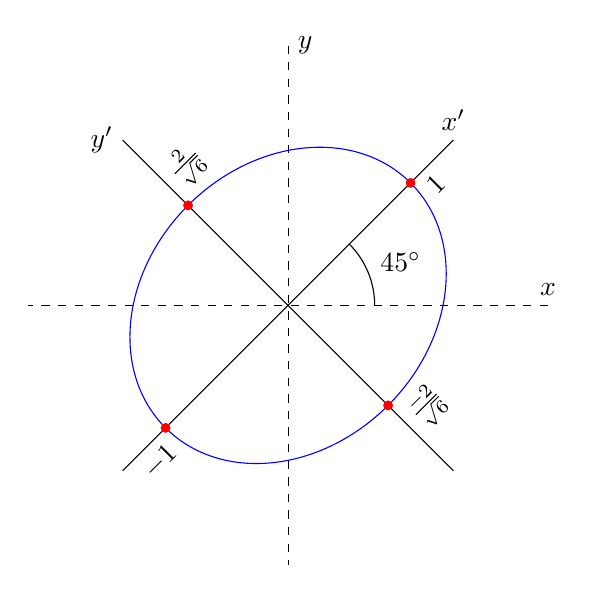
\begin{tikzpicture}[scale=1.1]
        \begin{scope}[dashed] 
            \draw (0,3) node[right]{$y$} -- (0,-3);
            \draw (3,0) node[above]{$x$} -- (-3,0);
        \end{scope}
        \begin{scope}[rotate=45] 
            \draw[blue] (0,0) circle (2 and 1.633); 
            \draw (0,2.7) node[left]{$y'$} --  (0,-2.7);
            \draw (2.7,0) node[above]{$x'$} -- (-2.7,0);
            \draw[red, fill=red] (0, 1.633) circle(0.05);
            \draw (0, 1.633) node[anchor=south west, rotate=45]{$\frac{2}{\sqrt{6}}$};
            \draw[red, fill=red] (0, -1.633) circle(0.05);
            \draw (0, -1.633) node[anchor=north west, rotate=45]{$\frac{-2}{\sqrt{6}}$};
            \draw[red, fill=red] (2, 0) circle(0.05);
            \draw (2, 0) node[anchor=north west, rotate=45]{$1$};
            \draw[red, fill=red] (-2, 0) circle(0.05);
            \draw (-2, 0) node[anchor=north east, rotate=45]{$-1$};
        \end{scope}

        \draw (1, 0) arc (0: 45: 1);
        \draw (1.3, 0.5) node {$45^{\circ}$};
    \end{tikzpicture}
    \caption{Ellipsen som beskrivs $5x^2-2xy+5y^2-4=0$}
\end{figure}

\newpage

\begin{thr}
    Klassificera (d.v.s. ange den geometriska betydelsen) andragradsuttrycket $5x^2-2xy+5y^2-2\sqrt{2}x+3\sqrt{2}y-4=0$ och skissera det i xy-planet.
\end{thr}

\vskip 0.3cm

Enligt uppgift 4 kan vi beskriva första delen av uttrycket $5x^2-2xy+5y^2$ som $4(x^{'})^2+6(y^{'})^2$ där vi har följande basbyte och basbytesmatris $T$:

$$
\begin{pmatrix}
    x \\
    y
\end{pmatrix}
=
T
\begin{pmatrix}
    x^{'} \\
    y^{'}
\end{pmatrix}
\Ekv
\begin{pmatrix}
    x \\
    y
\end{pmatrix}
=
\begin{pmatrix}
    \frac{1}{\sqrt{2}} & \frac{-1}{\sqrt{2}} \\
    \frac{1}{\sqrt{2}} & \frac{1}{\sqrt{2}}
\end{pmatrix}
\begin{pmatrix}
    x^{'} \\
    y^{'}
\end{pmatrix}
$$

\vskip 0.3cm

Vi kan även skriva andra delen av uttrycket, förutom konstanten 4, med basbytet på följande vis:

$$
-2\sqrt{2}x+3\sqrt{2}y=
\begin{pmatrix}
    -2\sqrt{2} & 3\sqrt{2}
\end{pmatrix}
\begin{pmatrix}
    x \\
    y
\end{pmatrix}
$$

\vskip 0.3cm

$$
\therefore
\;
-2\sqrt{2}x+3\sqrt{2}y=
\begin{pmatrix}
    -2\sqrt{2} & 3\sqrt{2}
\end{pmatrix}
\begin{pmatrix}
    x \\
    y
\end{pmatrix}
=
\begin{pmatrix}
    -2\sqrt{2} & 3\sqrt{2}
\end{pmatrix}
\begin{pmatrix}
    \frac{1}{\sqrt{2}} & \frac{-1}{\sqrt{2}} \\
    \frac{1}{\sqrt{2}} & \frac{1}{\sqrt{2}}
\end{pmatrix}
\begin{pmatrix}
    x^{'} \\
    y^{'}
\end{pmatrix}
$$

$$
=
\begin{pmatrix}
    -2+3 & 2+3
\end{pmatrix}
\begin{pmatrix}
    x^{'} \\
    y^{'}
\end{pmatrix}
=
\begin{pmatrix}
    1 & 5 
\end{pmatrix}
\begin{pmatrix}
    x^{'} \\
    y^{'}
\end{pmatrix}
=
x^{'}+5y^{'}
$$

\vskip 0.3cm

$$
\therefore
\;
5x^2-2xy+5y^2-2\sqrt{2}x+3\sqrt{2}y-4=0 
\Ekv
4(x^{'})^2+6(y^{'})^2+x^{'}+5y^{'}=4
$$

$$
\Ekv_{Kvadratkomplettering}
\;\;
4(x^{'}+\frac{1}{8})^2-\frac{1}{16}+6(y^{'}+\frac{5}{12})^2-\frac{25}{24}=4
$$

$$
\Ekv
4(x^{'}+\frac{1}{8})^2+6(y^{'}+\frac{5}{12})^2=\frac{245}{48}
\Ekv
\frac{(x^{'}+\frac{1}{8})^2}{(\sqrt{\frac{245}{192}})^2}+\frac{(y^{'}+\frac{5}{12})^2}{(\sqrt{\frac{245}{288}})^2}=1
$$

\vskip 0.3cm

$\therefore \;$ Andragradsuttrycket $5x^2-2xy+5y^2-2\sqrt{2}x+3\sqrt{2}y-4=0$ är ekvivalent med ellipsen som beskrivs av uttrycket $\frac{(x^{'}+\frac{1}{8})^2}{(\sqrt{\frac{245}{192}})^2}+\frac{(y^{'}+\frac{5}{12})^2}{(\sqrt{\frac{245}{288}})^2}=1$ där basbytet motsvarar en medurs rotation med 45\textdegree $\:$ vilket visades i uppgift 3. Detta skisseras i figuren på nästa sida:

\newpage

\begin{figure}[h]
    \centering
    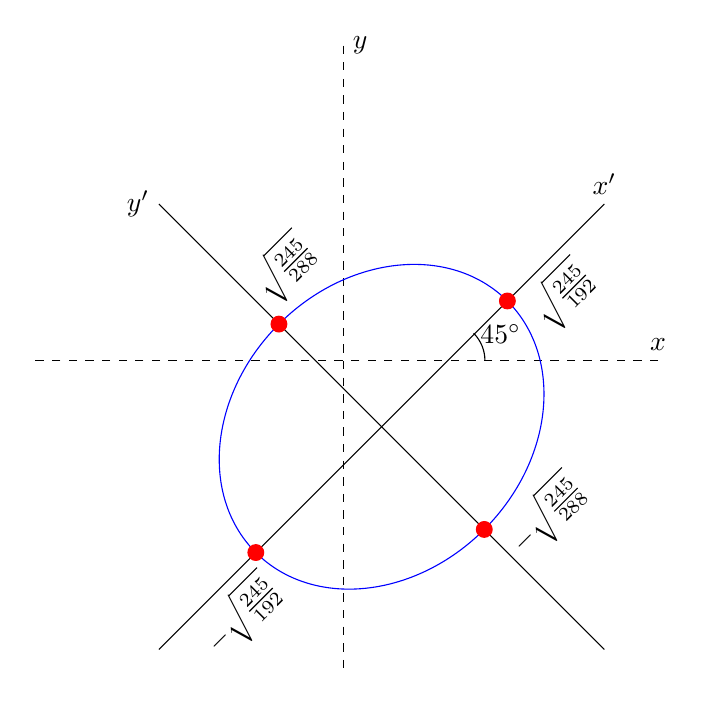
\begin{tikzpicture}[scale=2]
        \begin{scope}[dashed] 
            \draw (0,2) node[right]{$y$} -- (0,-2);
            \draw (2,0) node[above]{$x$} -- (-2,0);
        \end{scope}
        \begin{scope}[rotate=45] 
            \draw[blue] (-0.125,-0.47) circle (1.1296 and 0.922); 
            \draw (-0.125,2-0.47) node[left]{$y'$} --  (-0.125,-2-0.47);
            \draw (2-0.125,-0.47) node[above]{$x'$} -- (-2-0.125,-0.47);

            \draw[red, fill=red] (-0.125, 0.922-0.47) circle(0.05);
            \draw (-0.125, 0.922-0.47) node[anchor=south west, rotate=45]{$\sqrt{\frac{245}{288}}$};
            \draw[red, fill=red] (-0.125, -0.922-0.47) circle(0.05);
            \draw (-0.125, -0.92-0.47) node[anchor=north west, rotate=45]{$-\sqrt{\frac{245}{288}}$};
            \draw[red, fill=red] (1.1296-0.125, -0.47) circle(0.05);
            \draw (1.1296-0.125, -0.47) node[anchor=north west, rotate=45]{$\sqrt{\frac{245}{192}}$};
            \draw[red, fill=red] (-1.1296-0.125, -0.47) circle(0.05);
            \draw (-1.1296-0.125, -0.47) node[anchor=north east, rotate=45]{$-\sqrt{\frac{245}{192}}$};
        \end{scope}

        \draw (0.9, 0) arc (0: 45: 0.245);
        \draw (1, 0.17) node {$45^{\circ}$};
    \end{tikzpicture}
    \caption{Ellipsen som beskrivs av $5x^2-2xy+5y^2-2\sqrt{2}x+3\sqrt{2}y-4=0$}
\end{figure}

\end{document}
